\documentclass[tikz,border=4pt]{standalone}
\usepackage{tikz}
\usetikzlibrary{arrows.meta,positioning}
\begin{document}
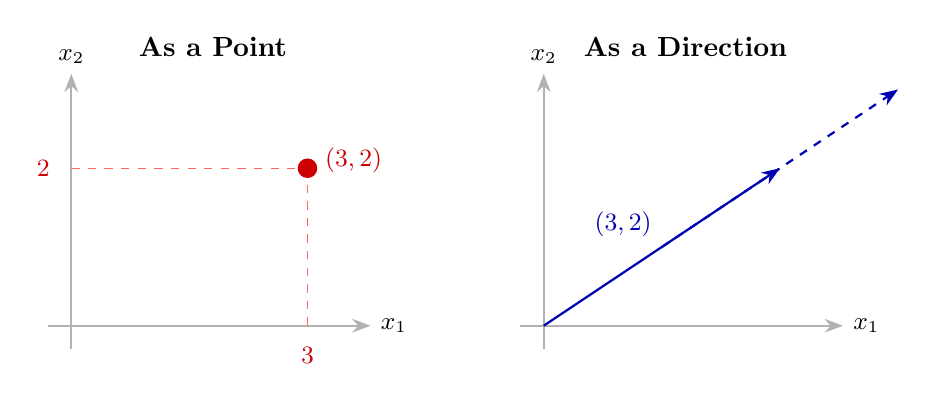
\begin{tikzpicture}[
    >=Stealth,
    axis/.style={->,gray!60,thick},
    vec/.style={->,thick},
    point/.style={circle,fill=#1,inner sep=2.5pt},
]
% === Left: vector as point ===
\begin{scope}[shift={(0,0)}]
    \node[font=\bfseries,anchor=south] at (1.8,3.3) {As a Point};
    \draw[axis] (-0.3,0) -- (3.8,0) node[right,font=\small,black] {$x_1$};
    \draw[axis] (0,-0.3) -- (0,3.2) node[above,font=\small,black] {$x_2$};
    \node[point=red!80!black] (p) at (3,2) {};
    \draw[dashed,red!60,thin] (3,0) -- (p);
    \draw[dashed,red!60,thin] (0,2) -- (p);
    \node[red!80!black,font=\small,right] at (3.1,2.1) {$(3,2)$};
    \node[font=\small,red!80!black,below] at (3,-0.15) {$3$};
    \node[font=\small,red!80!black,left] at (-0.15,2) {$2$};
\end{scope}

% === Right: vector as direction ===
\begin{scope}[shift={(6,0)}]
    \node[font=\bfseries,anchor=south] at (1.8,3.3) {As a Direction};
    \draw[axis] (-0.3,0) -- (3.8,0) node[right,font=\small,black] {$x_1$};
    \draw[axis] (0,-0.3) -- (0,3.2) node[above,font=\small,black] {$x_2$};
    \draw[vec,blue!70!black] (0,0) -- (3,2)
        node[midway,above left,font=\small,blue!70!black] {$(3,2)$};
    \draw[vec,blue!70!black,dashed] (1.5,1) -- (4.5,3);
\end{scope}
\end{tikzpicture}
\end{document}
